% loman.tex --- A technical description of the Loman library
%
% Build with:
%   pdflatex loman.tex
%   pdflatex loman.tex      (twice, for cross-references)
%
% Only standard TeX Live packages are used; no external .bib file is required.

\documentclass[11pt,a4paper]{article}

\usepackage[T1]{fontenc}
\usepackage[utf8]{inputenc}
\usepackage{lmodern}
\usepackage[margin=2.6cm]{geometry}
\usepackage{amsmath,amssymb}
\usepackage{booktabs}
\usepackage{longtable}
\usepackage{xcolor}
\usepackage{listings}
\usepackage{tikz}
\usetikzlibrary{arrows.meta,positioning,shapes.geometric,fit,backgrounds}
\usepackage{caption}
\usepackage[hidelinks]{hyperref}

%------------------------------------------------------------------
% Listings style for Python
%------------------------------------------------------------------
\definecolor{codegray}{gray}{0.96}
\definecolor{codekw}{RGB}{0,80,160}
\definecolor{codestr}{RGB}{160,60,60}
\definecolor{codecom}{RGB}{100,110,100}

\lstdefinestyle{py}{
  language=Python,
  backgroundcolor=\color{codegray},
  basicstyle=\ttfamily\small,
  keywordstyle=\color{codekw}\bfseries,
  stringstyle=\color{codestr},
  commentstyle=\color{codecom}\itshape,
  showstringspaces=false,
  breaklines=true,
  columns=fullflexible,
  frame=single,
  framerule=0pt,
  xleftmargin=0.6em,
  framexleftmargin=0.6em,
  literate={'}{{\textquotesingle}}1,
}
\lstset{style=py}

%------------------------------------------------------------------
% State colours, taken from loman.visualization.ColorByState
%------------------------------------------------------------------
\definecolor{stPlaceholder}{HTML}{F97306}
\definecolor{stUninit}{HTML}{0343DF}
\definecolor{stStale}{HTML}{FFFF14}
\definecolor{stComputable}{HTML}{9DFF00}
\definecolor{stUptodate}{HTML}{15B01A}
\definecolor{stError}{HTML}{E50000}
\definecolor{stPinned}{HTML}{BF77F6}

\newcommand{\swatch}[1]{\tikz[baseline=-0.5ex]\draw[fill=#1,draw=black!45]
  (0,0) rectangle (0.85em,0.85em);}

\newcommand{\loman}{\textsc{Loman}}
\newcommand{\code}[1]{\texttt{#1}}

%------------------------------------------------------------------
\title{\loman: Dependency-Aware Computation Graphs\\ for Partial Recalculation in Python}

\author{A technical description of the \code{loman} repository}
\date{\today}

\begin{document}
\maketitle

\begin{abstract}
\loman{} is a Python library that represents a computation as an explicit
directed acyclic graph (DAG) of named values. Each node is either an
\emph{input}, whose value is supplied from outside, or a \emph{calculation},
whose value is produced by a Python function of other nodes. \loman{} tracks a
per-node lifecycle state, so that when an input changes or a function is
redefined, only the affected part of the graph is invalidated and only the
part actually required by a requested output is recomputed. The library
additionally provides hierarchical node namespaces and composable sub-graphs
(\emph{blocks}), non-mutating validation and execution planning, pluggable
executors, JSON and \code{dill} serialization of an entire computation
including intermediate values, and GraphViz-based visualization in which node
colour encodes state. This document describes the computation model, the
state machine that drives partial recalculation, the public API, the internal
architecture of the repository, and the engineering practices that surround
it.
\end{abstract}

\tableofcontents
\bigskip

%==================================================================
\section{Introduction}
%==================================================================

Most non-trivial analytical systems are, at heart, a set of values that depend
on other values. A portfolio valuation depends on positions and prices;
prices depend on a market data pull; the pull depends on a run date and a
database connection. In practice this dependency structure is usually left
implicit, encoded in the ordering of statements in a \code{main} function or in
the ordering of tasks in a scheduler. \loman{} makes the structure explicit
and executable.

The library's own introduction \cite{lomandocs} motivates it from two
directions, both drawn from production experience with systems that consume
data from many independent sources:

\begin{description}
  \item[Scheduled batch systems.] When a required input is late or missing,
  downstream scheduled tasks may run anyway and silently produce wrong
  results. When a re-run is needed, it is often unclear which steps must be
  repeated, so operators re-run everything. A large share of the operational
  cost of such systems is the spare capacity kept purely for improvised
  re-runs.
  \item[Single programs.] A complex calculation is rarely correct on the first
  attempt. If each iteration re-pulls large data sets and re-runs expensive
  steps that could not have changed, the developer's iteration rate --- not
  the machine --- becomes the limiting factor.
\end{description}

\loman{}'s answer to both is the same: hold the computation as a graph, track
what is current and what is not, and recompute exactly the difference. The
analogy the documentation itself offers is \code{make} for calculations, or the
dependency tree behind a spreadsheet.

The remainder of this document is organised as follows. Section~\ref{sec:model}
introduces the computation model. Section~\ref{sec:states} describes the state
machine that makes partial recalculation possible. Section~\ref{sec:api}
surveys the public API. Sections~\ref{sec:hierarchy}--\ref{sec:viz} cover
hierarchical namespaces and blocks, validation and planning, execution,
serialization, and visualization. Section~\ref{sec:repo} describes the
repository layout and engineering practices, and Section~\ref{sec:limits}
discusses limitations and directions for future work.

%==================================================================
\section{The computation model}\label{sec:model}
%==================================================================

A \loman{} computation is an instance of the \code{Computation} class. It owns
a \code{networkx} directed graph \cite{networkx} whose vertices are nodes and
whose edges record parameter flow: an edge $u \to v$ means that the value of
$u$ is supplied as an argument to the function of $v$. Each edge carries a
\code{param} attribute recording \emph{which} argument --- either a positional
index or a keyword name --- so that the same predecessor can feed several
parameters, and so that arguments can be re-bound without disturbing the rest
of the graph.

\subsection{Nodes}

A node carries the attributes listed in Table~\ref{tab:nodeattrs}. Two node
kinds matter conceptually:

\begin{itemize}
  \item An \textbf{input node} has no function. Its value arrives from outside
  via \code{insert}, or via the \code{value=} argument of \code{add\_node}.
  \item A \textbf{calculation node} has a function. Its value is the result of
  calling that function with values drawn from its predecessors.
\end{itemize}

A third, transient kind exists: a \textbf{placeholder}. When a function names a
parameter for which no node yet exists, \loman{} creates the node immediately
in the \code{PLACEHOLDER} state, so that the graph is always structurally
complete even while it is being built out of order. A placeholder is not an
error at construction time; it becomes one only if a computation depends on it.

\begin{table}[t]
\centering
\caption{Node attributes stored on the underlying \code{networkx} graph
(\code{loman/consts.py}).}
\label{tab:nodeattrs}
\begin{tabular}{@{}lp{9.6cm}@{}}
\toprule
Attribute & Meaning \\
\midrule
\code{value}     & The current value of the node. \\
\code{state}     & A member of the \code{States} enumeration (Section~\ref{sec:states}). \\
\code{func}      & The callable for a calculation node; \code{None} for an input. \\
\code{args}      & Constant positional arguments bound at definition time. \\
\code{kwds}      & Constant keyword arguments bound at definition time. \\
\code{group}     & Optional subgraph grouping used for rendering. \\
\code{tag}       & A set of user and system tags (e.g.\ \code{\_\_serialize\_\_}). \\
\code{style}     & Optional named style used for rendering. \\
\code{timing}    & Start, end and elapsed time of the most recent evaluation. \\
\code{executor}  & Name of the executor on which the node should run. \\
\code{converter} & Optional callable applied to a value on insertion. \\
\bottomrule
\end{tabular}
\end{table}

\subsection{Binding arguments to nodes}

By default \loman{} binds function parameters to nodes \emph{by name}, using
introspection of the function signature. A function \code{def f(a, b)}
registered as node \code{c} therefore consumes nodes \code{a} and \code{b}. This
convention keeps simple graphs almost free of boilerplate:

\begin{lstlisting}
from loman import Computation

comp = Computation()
comp.add_node('a', value=1)              # input node, given a value
comp.add_node('b', lambda a: a + 1)      # b depends on a
comp.add_node('c', lambda a, b: 2 * a)   # c declares a and b
comp.add_node('d', lambda b, c: b + c)   # d depends on b and c
comp.add_node('e', lambda c: c + 1)      # e depends on c

comp.compute('d')          # computes a, b, c, d --- but not e
comp.to_dict()
# {'a': 1, 'b': 2, 'c': 2, 'd': 4, 'e': None}
\end{lstlisting}

The convention can always be overridden. The \code{kwds} argument re-maps a
parameter to a differently named node, read as ``take parameter \emph{key} from
node \emph{value}''; \code{args} binds parameters positionally to a list of
nodes; and \code{C(\ldots)} (an alias for \code{ConstantValue}) binds a literal
rather than a node, so that a constant does not need a node of its own.
Introspection can be suppressed entirely with \code{inspect=False}, in which case
\code{args} and \code{kwds} must be supplied --- useful both for callables that
do not expose a signature and for hot paths where introspection cost matters.

\begin{figure}[t]
\centering
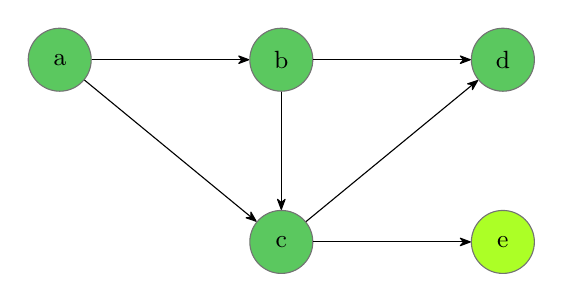
\begin{tikzpicture}[
  >={Stealth[round]},
  node distance=1.5cm and 2.0cm,
  every node/.style={font=\small},
  nd/.style={circle,draw=black!55,minimum size=8mm,fill=stUptodate!70},
  sk/.style={circle,draw=black!55,minimum size=8mm,fill=stComputable!85},
]
  \node[nd] (a) {a};
  \node[nd,right=of a] (b) {b};
  \node[nd,below=of b] (c) {c};
  \node[nd,right=of b] (d) {d};
  \node[sk,right=of c] (e) {e};

  \draw[->] (a) -- (b);
  \draw[->] (a) -- (c);
  \draw[->] (b) -- (c);
  \draw[->] (b) -- (d);
  \draw[->] (c) -- (d);
  \draw[->] (c) -- (e);
\end{tikzpicture}
\caption{The graph built by the example above, after \code{comp.compute('d')}.
Dark green nodes are \code{UPTODATE}. Node \code{e} was never requested, so it
was never evaluated; it sits at \code{COMPUTABLE} (light green), ready to run
because its only predecessor \code{c} is current. Requesting \code{d} pulls
exactly its ancestors and nothing else.}
\label{fig:dag}
\end{figure}

\subsection{Pull, not push}

\loman{} is demand-driven. Inserting a value does not trigger any calculation;
it only marks the affected region of the graph as out of date. Work happens
when the user asks for it, through \code{compute(name)} for a specific target,
\code{compute\_all()} for everything reachable, or the \code{comp.x.\emph{name}}
accessor, which computes a node and returns its value in one step. This is
what allows a graph to carry many nodes that are never evaluated: the
documentation explicitly recommends defining a node for every input, result or
intermediate that one might plausibly want to inspect, since unused nodes cost
nothing to leave in place.

%==================================================================
\section{States and partial recalculation}\label{sec:states}
%==================================================================

The state machine is the core of the library. Every node holds one of the
seven states in Table~\ref{tab:states}, and every mutation of the graph is
defined by its effect on states.

\begin{table}[t]
\centering
\caption{The \code{States} enumeration, with the colours used when a graph is
drawn.}
\label{tab:states}
\begin{tabular}{@{}llp{8.6cm}@{}}
\toprule
& State & Meaning \\
\midrule
\swatch{stPlaceholder} & \code{PLACEHOLDER}   & Referenced as a dependency but never defined. \\
\swatch{stUninit}      & \code{UNINITIALIZED} & Defined, but has never held a value. \\
\swatch{stStale}       & \code{STALE}         & Holds an old value that is no longer trustworthy. \\
\swatch{stComputable}  & \code{COMPUTABLE}    & Not current, but every predecessor is current: ready to run. \\
\swatch{stUptodate}    & \code{UPTODATE}      & Value reflects the current inputs and functions. \\
\swatch{stError}       & \code{ERROR}         & The most recent evaluation raised; the exception and traceback are stored as the value. \\
\swatch{stPinned}      & \code{PINNED}        & Value is held fixed by the user and is immune to invalidation. \\
\bottomrule
\end{tabular}
\end{table}

\subsection{Transitions}

Two internal operations generate almost all transitions.

\paragraph{Invalidation.} \code{\_set\_descendents} walks forward from a node
and marks every reachable descendant \code{STALE}. Crucially, the walk stops at
\code{PINNED} nodes: a pinned node and everything behind it are shielded from
invalidation. Invalidation is triggered by inserting a value, by a successful
evaluation (which staleness-marks everything downstream before the new value is
propagated), by an evaluation that raises, and by redefining a node with
\code{add\_node}.

\paragraph{Readiness.} \code{\_try\_set\_computable} examines a single node: if
it has a function, is not pinned, and every predecessor is \code{UPTODATE} or
\code{PINNED}, it becomes \code{COMPUTABLE}. This is the only route into the
runnable set, and it is re-evaluated for the successors of every node that
becomes current.

\begin{figure}[t]
\centering
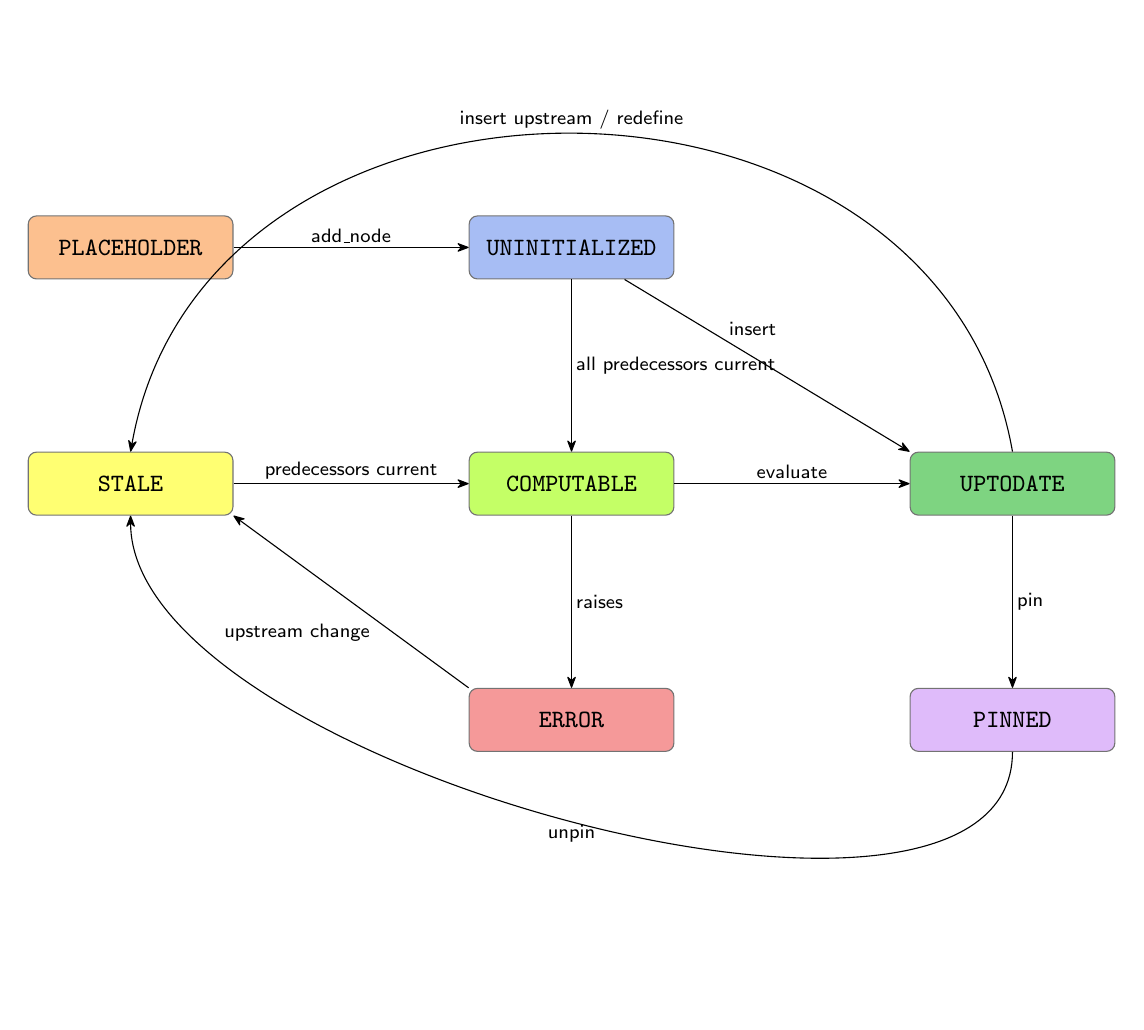
\begin{tikzpicture}[
  >={Stealth[round]},
  every node/.style={font=\small},
  st/.style={rounded corners=3pt,draw=black!55,minimum height=8mm,
             minimum width=26mm,align=center,font=\small\ttfamily},
]
  \node[st,fill=stPlaceholder!45] (ph)     at (0,0)      {PLACEHOLDER};
  \node[st,fill=stUninit!35]      (uninit) at (5.6,0)    {UNINITIALIZED};
  \node[st,fill=stStale!60]       (stale)  at (0,-3.0)   {STALE};
  \node[st,fill=stComputable!60]  (comp)   at (5.6,-3.0) {COMPUTABLE};
  \node[st,fill=stUptodate!55]    (up)     at (11.2,-3.0){UPTODATE};
  \node[st,fill=stError!40]       (err)    at (5.6,-6.0) {ERROR};
  \node[st,fill=stPinned!50]      (pin)    at (11.2,-6.0){PINNED};

  \tikzset{lb/.style={font=\scriptsize\sffamily,inner sep=1.5pt}}

  \draw[->] (ph)     -- node[lb,above]{add\_node} (uninit);
  \draw[->] (uninit) -- node[lb,right]{all predecessors current} (comp);
  \draw[->] (uninit) -- node[lb,above right,pos=0.35]{insert} (up.north west);
  \draw[->] (stale)  -- node[lb,above]{predecessors current} (comp);
  \draw[->] (comp)   -- node[lb,above]{evaluate} (up);
  \draw[->] (comp)   -- node[lb,right]{raises} (err);
  \draw[->] (up)     -- node[lb,right]{pin} (pin);
  \draw[->] (up.north) to[out=100,in=80,looseness=1.25]
        node[lb,above]{insert upstream / redefine} (stale.north);
  \draw[->] (err.north west) -- node[lb,below left,pos=0.4]{upstream change} (stale.south east);
  \draw[->] (pin.south) to[out=270,in=270,looseness=0.7]
        node[lb,below]{unpin} (stale.south);
\end{tikzpicture}
\caption{The principal state transitions. \code{insert} and node redefinition
mark descendants \code{STALE}; a stale node becomes \code{COMPUTABLE} as soon
as all of its predecessors are \code{UPTODATE} or \code{PINNED}. Invalidation
does not cross a \code{PINNED} node.}
\label{fig:states}
\end{figure}

\subsection{Why this yields minimal recomputation}

When \code{compute(target)} is called, \loman{} builds the ancestor set of the
target and then \emph{removes} from it every node that is already
\code{UPTODATE} or \code{PINNED}. Removing a current node also severs the paths
through it, so the traversal stops there: the value of a current node is taken
as given, and nothing behind it is revisited. What remains is exactly the set
of nodes whose values are unknown and required. That set is topologically
sorted and executed.

Two consequences follow directly. First, work is bounded below by the target's
ancestors and above by the stale frontier --- nothing outside the cone of
influence of the target is touched, which is why \code{e} in
Figure~\ref{fig:dag} is never evaluated. Second, the mechanism is agnostic to
\emph{why} something became stale: a new input value, a redefined function, an
unpinned override and a manually forced \code{set\_stale} all invalidate through
the same path, so ``I changed how this is calculated'' is as cheap and as
correct as ``I received new data''.

\subsection{Pinning and manual override}

\code{pin(name, value)} inserts a value and holds it. A pinned node ignores
upstream invalidation, which makes it possible to override an intermediate
result --- to patch a bad price, or to test a hypothesis --- and recompute
downstream without the override being immediately washed away by the upstream
values that contradict it. \code{unpin} restores normal behaviour by marking
the node and its descendants \code{STALE}, so that the override is undone and
the affected region recalculates on the next request.

%==================================================================
\section{The public API}\label{sec:api}
%==================================================================

\subsection{Defining a computation}

The primary constructor is \code{add\_node}. Beyond \code{func}, \code{args},
\code{kwds} and \code{value}, it accepts \code{converter} (a callable applied to
inserted values), \code{serialize} (whether the node participates in
serialization), \code{group} and \code{style} (rendering hints), \code{tags}
(arbitrary labels, queryable via \code{nodes\_by\_tag}), \code{executor} (the
name of the executor to run on) and \code{metadata}.

For larger graphs, a declarative class-based form avoids repeated
\code{add\_node} calls. A class decorated with \code{@computation\_factory}
becomes a factory function; its members decorated with \code{@calc\_node}, or
assigned \code{input\_node(\ldots)} or \code{block(\ldots)}, become the nodes of
each computation the factory produces:

\begin{lstlisting}
from loman import calc_node, computation_factory, input_node

@computation_factory
class Pricing:
    spot = input_node()
    vol = input_node()

    @calc_node
    def variance(vol):
        return vol ** 2

    @calc_node
    def price(spot, variance):
        return spot * variance

comp = Pricing()        # a fresh Computation, wired up
comp.insert('spot', 100.0)
comp.insert('vol', 0.2)
comp.compute_all()
\end{lstlisting}

Related conveniences include \code{add\_named\_tuple\_expansion}, which
generates one extraction node per field of a \code{namedtuple}-valued node (so
that \code{node.field} can be depended on individually rather than the whole
tuple), and \code{add\_map\_node}, which applies a sub-computation to each
element of an iterable node in the manner of \code{map}, collecting either the
results or --- on failure --- copies of the sub-computations that failed, which
is precisely what one wants for debugging a partial failure.

\subsection{Inspecting a computation}

\loman{} is designed for interactive use, and offers several parallel access
paths. Methods \code{value}, \code{state}, \code{tags}, \code{styles},
\code{get\_timing} and the \code{[]} operator each accept a single name or a
list of names. Attribute-style views provide the same data with tab-completion
in IPython and Jupyter: \code{comp.v} for values, \code{comp.s} for states,
\code{comp.i} and \code{comp.o} for inputs and outputs, \code{comp.t} for tags,
\code{comp.tim} for timings, \code{comp.src} for source code, and \code{comp.x}
to compute-and-fetch. These views nest, so \code{comp.v.block.sub.node} is
equivalent to \code{comp.v['block/sub/node']}.

Whole-graph views are available as \code{to\_dict()} and \code{to\_df()}, the
latter returning a \code{pandas} \cite{pandas} frame of states and values.
Structural queries include \code{get\_inputs}, \code{get\_outputs},
\code{get\_ancestors}, \code{get\_descendents}, \code{get\_original\_inputs}
(the source nodes of the graph) and \code{get\_final\_outputs} (the sinks).
\code{restrict} prunes a computation to the sub-graph between a given set of
inputs and outputs. \code{get\_source} and \code{print\_source} recover the
source text of a node's function, which matters when inspecting a
deserialized graph whose code is no longer in front of you.

\subsection{Mutating a computation}

Nodes can be added, redefined by calling \code{add\_node} again with the same
name, deleted, renamed (singly or via a mapping), and repointed --- \code{repoint}
redirects every consumer of one node to another, which is the natural operation
for swapping a data source or splicing a mock into place. \code{link} creates
an alias node that forwards a value. \code{insert\_many} inserts a batch of
values, and \code{insert\_from} copies values across from another computation,
which is the usual way to seed a fresh graph from a serialized run.

%==================================================================
\section{Hierarchical namespaces and blocks}\label{sec:hierarchy}
%==================================================================

Node names are not restricted to strings. Internally every name is normalised
to a \code{NodeKey}, an immutable tuple of hashable parts rendered with a path
syntax, \code{a/b/c}. Parts that themselves contain a slash are quoted using
JSON escaping, so paths remain unambiguous. Because the parts need only be
hashable, tuples, dates and enumeration members are all valid names --- useful
when a graph is naturally indexed by something other than an identifier.

Paths give the graph a tree structure alongside its DAG structure, and the tree
is what \code{add\_block} exploits. A block is an entire \code{Computation}
grafted into another under a prefix:

\begin{lstlisting}
sub = Computation()
sub.add_node('x')
sub.add_node('y', lambda x: x * 2)

comp = Computation()
comp.add_node('source', value=21)
comp.add_block('leg1', sub, links={'x': 'source'})
comp.add_block('leg2', sub, links={'x': 'source'})
comp.compute('leg1')        # computes every node under leg1/
comp.v.leg1.y               # 42
\end{lstlisting}

Every node of the block is re-added under the prefix with its arguments
rewritten to the new namespace, preserving functions, groups, styles, tags,
converters and executor assignments. The \code{links} argument wires block
inputs to nodes in the host graph, and \code{keep\_values} controls whether the
block's current values come along with its structure. Because parameter name
resolution is relative to the enclosing block, a sub-graph written in isolation
composes without renaming. Blocks are addressable as units: \code{compute} on a
block path computes every node beneath it, and \code{draw(root=\ldots)} renders
a single block.

%==================================================================
\section{Validation and planning}\label{sec:plan}
%==================================================================

A distinctive and relatively recent feature is that \loman{} can answer
questions about what \emph{would} happen without doing it. Both APIs in
\code{loman/planning.py} are pure: they read the graph and return frozen
dataclasses, executing no user function and mutating no state.

\code{validate()} returns a \code{ValidationReport} recording dependency cycles
(as strongly connected components), placeholder nodes, uninitialized inputs,
error nodes, and nodes assigned to an executor that is not configured. Two
derived properties summarise it: \code{is\_valid} covers structural problems
(cycles, placeholders, missing executors) and \code{is\_ready} additionally
requires that all inputs are present and no node is in error.

\code{plan(targets)} returns an \code{ExecutionPlan}: the topologically ordered
list of nodes that would run, the nodes taken as already current, the blocked
nodes together with the specific blockers responsible and a human-readable
reason for each, and the executor each node would be dispatched to.
\code{is\_feasible} reports whether every requested target can be brought up to
date. Both objects render as \code{pandas} frames via \code{to\_df()}, one row
per issue or per node:

\begin{lstlisting}
plan = comp.plan('report')
if not plan.is_feasible:
    print(plan.to_df())      # node, state, plan_status, order,
                             # executor, blocked_by, reason
\end{lstlisting}

The practical value is operational. A batch job can validate before it starts
and fail loudly with a precise diagnosis --- ``\code{prices} has not been
supplied, which blocks \code{valuation} and \code{report}'' --- rather than
running half-way and producing a plausible but wrong answer, which is exactly
the failure mode the introduction identifies in schedule-driven systems. The
same report drives a dry run: the plan tells an operator which steps a re-run
would actually repeat before any of them is paid for.

%==================================================================
\section{Execution}\label{sec:exec}
%==================================================================

Execution is driven by \code{\_compute\_nodes}, which submits work to
\code{concurrent.futures} executors and consumes completions as they arrive.
The loop is:

\begin{enumerate}
  \item Submit every node in the required set that is currently
  \code{COMPUTABLE}.
  \item Wait for the first completion.
  \item On success, store the value, record timing, mark descendants
  \code{STALE}, then test each successor for readiness and submit any that
  became \code{COMPUTABLE} and belong to the required set.
  \item On failure, set the node \code{ERROR} with the exception and formatted
  traceback as its value, and mark its descendants \code{STALE}.
  \item Repeat until no futures remain.
\end{enumerate}

The design has three noteworthy properties. Concurrency is implicit: any two
nodes that are simultaneously ready run simultaneously, so parallelism follows
from the shape of the graph rather than from user annotation. Failure is
contained: by default an exception does not abort the run, and the engine
proceeds as far as the remaining dependencies allow, so a single bad branch
does not deprive the user of the rest of the results. And because a node that
would be scheduled twice indicates a cycle, the loop detects re-entry and
raises \code{LoopDetectedError}, guarding an invariant that the topological sort
assumes.

Each \code{Computation} carries a \code{default\_executor} --- a
single-threaded \code{ThreadPoolExecutor} unless overridden --- and a named
\code{executor\_map}. A node's \code{executor} attribute selects from the map,
so I/O-bound nodes can be routed to a wide thread pool while CPU-bound nodes
go to a process pool, all within one graph. \code{raise\_exceptions=True} opts
out of failure containment for callers who prefer to propagate.

%==================================================================
\section{Serialization}\label{sec:serial}
%==================================================================

A computation can be written whole --- structure, functions, states and
values --- and read back. Two formats are supported.

\code{write\_dill} / \code{read\_dill} use \code{dill} \cite{dill} to pickle the
graph. This handles almost any Python object, including closures, at the cost
of a binary, version-sensitive format that requires trusting the source of the
file.

\code{write\_json} / \code{read\_json} use a transformer framework in
\code{loman/serialization/}. A \code{Transformer} holds a registry of type
handlers, and dispatch is by exact type or registered subtype, with classes
ordered so that the most specific handler wins. Handlers ship for
\code{numpy} \cite{numpy} arrays, enumerations, \code{attrs} classes and
dataclasses, and user types can register by implementing a
\code{CustomTransformer} or the \code{Transformable} protocol. Functions are
stored by importable module path, which means a lambda cannot be serialized
and raises \code{SerializationError} --- a deliberate constraint that pushes
users towards module-level functions that a reader can actually resolve. The
result is a plain, human-readable JSON document that can be inspected in a text
editor without running any code.

The \code{serialize=False} flag on \code{add\_node} excludes a node from
serialization while preserving it structurally: the node reappears
\code{UNINITIALIZED} on load. This is how connection objects, credentials and
licensed data are kept out of the artefact. The recommended pattern for
database access is a pair of non-serialized nodes for the engine and metadata
object, with every data-access node depending on them --- a form of dependency
injection, and one that \code{inject\_dependencies} supports directly.

Serialization is what turns the graph into an operational tool. A batch job
that serializes on completion, or on failure, leaves behind a complete record:
every input, every intermediate, every state, and the traceback of whatever
went wrong. Post-mortem debugging becomes an interactive session against that
file, and recovery becomes an \code{insert} of the corrected input followed by a
\code{compute} that repeats only what is genuinely affected.

%==================================================================
\section{Visualization}\label{sec:viz}
%==================================================================

\code{comp.draw()} renders the graph through GraphViz via \code{pydotplus}.
Rendering is organised as composable \code{NodeFormatter} objects:
\code{ColorByState} applies the palette of Table~\ref{tab:states};
\code{ColorByTiming} shades by elapsed time using a \code{matplotlib}
\cite{matplotlib} colormap, which turns the graph into a profile;
\code{ShapeByType} distinguishes inputs from calculations; and
\code{StandardGroup} maps the \code{group} attribute and the path hierarchy onto
GraphViz subgraph clusters. A \code{StandardStylingOverrides} formatter applies
per-node styles last, so explicit user intent wins.

Large graphs are managed through \code{NodeTransformations}: \code{CONTRACT},
\code{COLLAPSE} and \code{EXPAND} control whether a block is drawn as a single
composite node or opened up, with pattern and wildcard matching to select
regions, and automatic expansion of the ancestors of anything expanded.
Because \code{Computation} implements \code{\_repr\_svg\_}, a computation
displays as a picture simply by being the last expression in a Jupyter cell;
the state colouring then makes the current condition of a large pipeline
readable at a glance.

%==================================================================
\section{Repository structure and engineering practice}\label{sec:repo}
%==================================================================

The distributable package lives under \code{src/loman/} and comprises roughly
3{,}700 lines of Python across the modules in Table~\ref{tab:modules}. It
targets Python 3.11 and above and depends on \code{networkx}, \code{pandas},
\code{numpy}, \code{matplotlib}, \code{pydotplus}, \code{dill}, \code{attrs}
and \code{decorator}.

\begin{table}[t]
\centering
\caption{Modules of the \code{loman} package.}
\label{tab:modules}
\begin{tabular}{@{}llp{7.4cm}@{}}
\toprule
Module & Lines & Responsibility \\
\midrule
\code{computeengine.py}   & 2084 & \code{Computation}, node definition, state transitions, execution, blocks, decorators. \\
\code{visualization.py}   &  675 & \code{GraphView}, node formatters, GraphViz output. \\
\code{nodekey.py}         &  286 & \code{NodeKey}, path parsing and hierarchy navigation. \\
\code{planning.py}        &  252 & Non-mutating validation and execution planning. \\
\code{serialization/}     & ---  & Transformer registry, JSON reader and writer. \\
\code{util.py}            &  147 & Attribute views, signature inspection helpers. \\
\code{graph\_utils.py}    &   68 & Graph helper routines. \\
\code{exception.py}       &   72 & Exception hierarchy rooted at \code{ComputationError}. \\
\code{consts.py}          &   52 & \code{States} and attribute-name constants. \\
\code{compat.py}          &   38 & Compatibility shims. \\
\bottomrule
\end{tabular}
\end{table}

Two conventions in the codebase are worth noting because they shape how it
reads. Node and edge attribute names are constants in \code{consts.py} rather
than string literals, so the schema of the underlying graph is stated in one
place. And exceptions form a single hierarchy under \code{ComputationError},
with the historical \code{\ldots Exception} spellings retained as aliases ---
one instance of a broader pattern in which the public surface is extended
without breaking existing callers, as with \code{ComputationFactory} aliasing
\code{computation\_factory}.

The project is managed with \code{uv} and \code{hatch}, linted and formatted
with \code{ruff}, type-checked with \code{mypy}, and security-scanned with
\code{bandit}. Tests are written with \code{pytest} across thirteen modules
that mirror the source layout, including a dedicated typing test. Pre-commit
hooks, a devcontainer, GitHub Codespaces support and Marimo notebooks for the
worked examples --- interest rate swap pricing, portfolio valuation and CDO
modelling --- round out the developer environment. Documentation is built with
MkDocs and published to Read the Docs.

%==================================================================
\section{Related work}\label{sec:related}
%==================================================================

\loman{} sits between several established categories and is best understood by
contrast with each.

\paragraph{Build systems.} \code{make} \cite{make} and its descendants share
the central idea: a dependency graph plus a currency test yields minimal
rebuilds. \loman{}'s currency test is explicit state rather than file
timestamps, and its units are in-memory Python values rather than files, which
removes the serialization round-trip that a file-based tool imposes on every
intermediate.

\paragraph{Workflow orchestrators.} Airflow \cite{airflow}, Luigi, Prefect and
Dagster also model pipelines as DAGs, but they are oriented towards scheduled,
distributed, long-running tasks with durable state in an external store.
\loman{} is a library, not a service: a computation is an ordinary Python
object that lives in a process, can be held in a notebook, and can be pickled
to a file. The repository does contain design plans for an Airflow integration
and for an AnyWidget-based UI, positioning \loman{} as the in-process
calculation kernel underneath such systems rather than a replacement for them.

\paragraph{Parallel computing frameworks.} Dask \cite{dask} builds task graphs
to schedule large computations across cores and clusters. Its graphs are
typically constructed per-invocation and discarded; \loman{}'s graph is a
persistent, inspectable, mutable object whose entire point is to survive
between invocations and remember what is already known. The concerns are
complementary --- \loman{} decides \emph{what} must run, a scheduler decides
\emph{where}.

\paragraph{Spreadsheets and reactive systems.} A spreadsheet's recalculation
engine is the closest everyday analogue, and \loman{} borrows its model:
named cells, a dependency graph, automatic invalidation. The differences are
that \loman{}'s cells hold arbitrary Python objects rather than scalars, and
that recalculation is pull-based and explicit, which matters when a single node
may take minutes to evaluate.

%==================================================================
\section{Limitations and future work}\label{sec:limits}
%==================================================================

Several limitations are acknowledged in the project's own documentation or
follow from its design.

\begin{itemize}
  \item \textbf{Per-node overhead.} Executing a node costs more than executing
  a line of Python. The guidance is to make a node of every value one might
  want to inspect, alter, or compute differently --- and no finer. The
  documentation also notes that determining computable nodes has not been
  optimised, leaving a linear cost in the number of unused nodes that is
  incidental rather than fundamental.

  \item \textbf{Value-blind invalidation.} Staleness is structural. A node is
  invalidated because an ancestor changed, not because the change altered its
  result. Inserting a value identical to the previous one still invalidates
  downstream. Content-addressed hashing of inputs would permit early cut-off,
  at the cost of requiring values to be hashable or comparable.

  \item \textbf{In-process scope.} A computation lives in one process. There
  is no built-in distributed execution and no persistent cache shared across
  runs; recovery across process boundaries goes through serialization.

  \item \textbf{Serialization constraints.} JSON serialization cannot capture
  lambdas or closures, and \code{dill} trades that flexibility for a binary
  format that must not be loaded from untrusted sources.

  \item \textbf{Introspection-based binding.} Binding parameters by name is
  concise but couples a function's parameter names to node names. Refactoring
  a parameter name silently re-points a dependency unless \code{kwds} is used,
  which is a real hazard in a large graph.
\end{itemize}

The changelog and design documents point at the active directions: an Airflow
extra that would let a \loman{} graph be driven by an external scheduler, and a
\code{loman[ui]} extra providing an interactive AnyWidget view of a live
computation. Both extend the same idea --- an explicit, inspectable graph ---
outward to the systems around it.

%==================================================================
\section{Conclusion}\label{sec:conclusion}
%==================================================================

\loman{}'s contribution is not a novel algorithm; dependency graphs and minimal
rebuilds are old ideas. Its contribution is placing that machinery inside a
Python process at a granularity the user chooses, and pairing it with the
facilities that make the resulting graph useful in practice: state that is
visible and colour-coded, plans that can be inspected before work is done,
serialization that captures a whole run for post-mortem analysis, and pinning
that lets a human override an intermediate and see the consequences propagate.

The result addresses both problems set out in the introduction with one
mechanism. For batch systems, the graph refuses to compute on absent inputs,
explains what is blocked and why, and records enough to diagnose a failure
after the fact and resume from it rather than restart. For interactive
research, changing a function invalidates only what that function reaches, so
the cost of an iteration falls to the cost of what actually changed. In both
cases the shift is the same: from an implicit, ordered sequence of steps to an
explicit, queryable structure that knows what it already knows.

%==================================================================
\begin{thebibliography}{99}

\bibitem{lomandocs}
Loman documentation and source repository.
\url{https://loman.readthedocs.io/} and
\url{https://github.com/janusassetallocation/loman}.

\bibitem{networkx}
A.~A. Hagberg, D.~A. Schult, and P.~J. Swart.
\newblock Exploring network structure, dynamics, and function using NetworkX.
\newblock In \emph{Proceedings of the 7th Python in Science Conference
  (SciPy2008)}, pp.~11--15, 2008.

\bibitem{pandas}
W.~McKinney.
\newblock Data structures for statistical computing in Python.
\newblock In \emph{Proceedings of the 9th Python in Science Conference}, 2010.

\bibitem{numpy}
C.~R. Harris et al.
\newblock Array programming with NumPy.
\newblock \emph{Nature}, 585:357--362, 2020.

\bibitem{matplotlib}
J.~D. Hunter.
\newblock Matplotlib: A 2D graphics environment.
\newblock \emph{Computing in Science \& Engineering}, 9(3):90--95, 2007.

\bibitem{dill}
M.~M. McKerns, L.~Strand, T.~Sullivan, A.~Fang, and M.~A.~G. Aivazis.
\newblock Building a framework for predictive science.
\newblock In \emph{Proceedings of the 10th Python in Science Conference}, 2011.

\bibitem{dask}
M.~Rocklin.
\newblock Dask: Parallel computation with blocked algorithms and task
  scheduling.
\newblock In \emph{Proceedings of the 14th Python in Science Conference}, 2015.

\bibitem{make}
S.~I. Feldman.
\newblock Make --- a program for maintaining computer programs.
\newblock \emph{Software: Practice and Experience}, 9(4):255--265, 1979.

\bibitem{airflow}
Apache Airflow.
\newblock \url{https://airflow.apache.org/}.

\end{thebibliography}

\end{document}
